\documentclass[tikz,border=10pt]{standalone}
\begin{document}
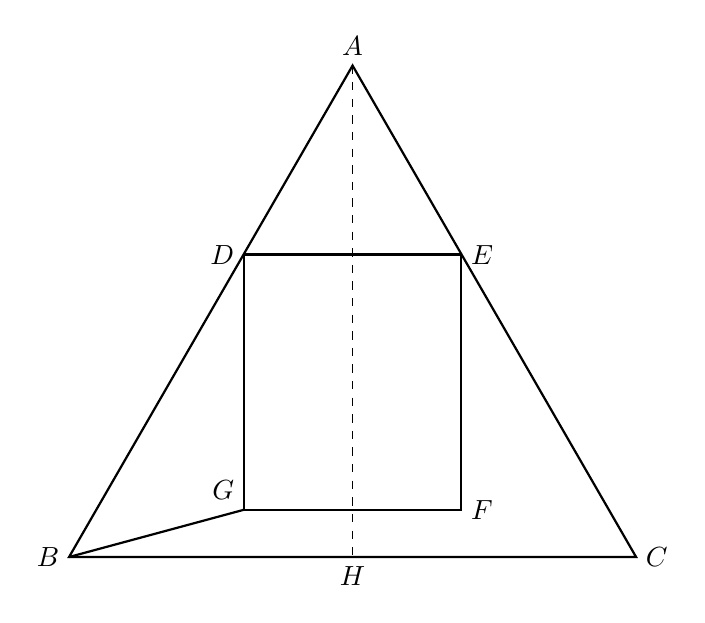
\begin{tikzpicture}[scale=1.2]
\coordinate (A) at (3,5.2);
\coordinate (B) at (0,0);
\coordinate (C) at (6,0);
\coordinate (D) at (1.85,3.2);
\coordinate (E) at (4.15,3.2);
\coordinate (G) at (1.85,0.5);
\coordinate (F) at (4.15,0.5);
\coordinate (H) at (3,0);

\draw[thick] (A) -- (B) -- (C) -- cycle;
\draw[thick] (D) -- (E);
\draw[thick] (D) -- (G) -- (F) -- (E);
\draw[thick] (B) -- (G);
\draw[dashed] (A) -- (H);

\node[above] at (A) {$A$};
\node[left] at (B) {$B$};
\node[right] at (C) {$C$};
\node[left] at (D) {$D$};
\node[right] at (E) {$E$};
\node[above left] at (G) {$G$};
\node[right] at (F) {$F$};
\node[below] at (H) {$H$};
\end{tikzpicture}
\end{document}
